\documentclass[11pt,a4paper]{article}
\usepackage[T1]{fontenc}
\usepackage[utf8]{inputenc}
\usepackage{lmodern}
\usepackage{microtype}
\usepackage[margin=2.3cm]{geometry}
\usepackage{booktabs,tabularx,array,graphicx,xcolor,enumitem,amsmath,float}
\usepackage[colorlinks=true,urlcolor=blue!50!black,linkcolor=blue!50!black]{hyperref}
\graphicspath{{figures/}}
\setlist{itemsep=2pt}
\newcolumntype{R}{>{\raggedleft\arraybackslash}X}
\newcommand{\code}[1]{\texttt{#1}}
\makeatletter\newcommand\rows[1]{\@@input #1 }\makeatother
\title{Moving-average distance and a volatility-scaled breakout on crypto\\[4pt]\large What was tested, how each strategy is computed, and what the data shows\\[2pt]\normalsize Data to 25 October 2026}
\date{25 October 2026}
\begin{document}
\maketitle

\noindent\fbox{\parbox{\dimexpr\linewidth-2\fboxsep}{\small
Every curve, table and number in this document is \textbf{simulated from historical data}, not the result of real trading.
Results were selected after many tests, on assets that still exist today, in a period when crypto mostly rose.
Expect lower returns in the future. This is a research record, not investment advice.}}

\section*{Summary}
\begin{itemize}
\item \textbf{MAD alone has no edge.} Plain, neutral-band, ADX-gated and volatility-normalised moving-average-distance (MAD) crossovers all fail
the Deflated Sharpe test: the best configuration per study scores below 0.36 against a bar of 0.95.
\item \textbf{Machine learning on top of MAD does not rescue it.} A logistic-regression and a gradient-boosting filter on each MAD trade, with
purged walk-forward validation, reach a best Deflated Sharpe of 0.20. A one-parameter rule on the size of the crossover jump (\code{dz}) does as well
as the model, but is unstable across settings.
\item \textbf{A MAD-free breakout does show a signal.} Buying after a fast, volatility-scaled move (12 bars, 2 standard deviations),
holding 24 bars of 4 hours, beats random entries on all 8 coins and in 7--8 of 9 calendar years. Pooled over 8 coins its compound
annual growth rate (CAGR) is 35.0\,\% against 33.2\,\% for Bitcoin buy-and-hold, with a maximum drawdown of $-26$\,\% against $-77$\,\%.
It is invested about 13\,\% of the time.
\item \textbf{It is a bear-market and sideways-market earner and a bull-market laggard.} In the 32 coin-years where buy-and-hold lost
(average $-42$\,\%), the rule averaged $+7.6$\,\%. In the 33 coin-years where buy-and-hold gained, it beat it in only 9\,\%.
\item \textbf{Status: promising, unproven.} The rule with a volume filter (k=12, H=24) is \emph{frozen} as of 25 October 2026 with a
pre-registered verdict (at least 100 forward trades). Nothing since the freeze can be scored yet. We recommend a \emph{watch-only} status,
not capital.
\end{itemize}

\tableofcontents
\clearpage

%% =====================================================================
\section{Question, data and conventions}
\subsection{The question}
The project began with one question: \emph{can moving-average distance (MAD) be a robust, standalone crypto trading strategy?} The answer
was no (Section~\ref{sec:mad}). The work then asked whether a filter or a different signal built on the same ideas could do better, and
how any claim should be tested so that luck is not mistaken for skill.

\subsection{Data}
\begin{itemize}
\item \textbf{Assets (8):} BTC, ETH, BNB, ADA, DOT, SOL, XRP, LINK, all against USDT on Binance spot. MATIC (renamed, 4-hour data to 2024) was used once as an
extra, non-surviving check.
\item \textbf{Frequency:} 4-hour bars (open, high, low, close, volume). For SOL, XRP and LINK the 4-hour bars were rebuilt from 1-hour bars (open
exact, closes within 0.36\,\% on a BTC check, volume up to 18\,\% off in the worst bar). On 25 October 2026 all assets were updated through
25 October 2026 from Binance's public klines endpoint, closed candles only. This also filled the BNB, ADA and DOT gap (their files had ended in May 2024).
\item \textbf{Sample:} between April 2018 and October 2026 depending on the coin (DOT and SOL start in August 2020, LINK in January 2019).
\item \textbf{Survivorship bias.} Seven of the eight coins are still listed and several rose 20 to 70 times. A long-only momentum rule
tested on survivors is flattered. MATIC does not repair this.
\end{itemize}

\subsection{Trading conventions}
\begin{itemize}
\item \textbf{Timing:} a signal uses information available strictly before the bar it trades on. Entry and exit are at the \emph{open} of a bar.
No indicator uses the high, low or close of the bar being traded.
\item \textbf{Costs:} 0.1\,\% of the traded value on each side, so a round trip costs about 0.2\,\%. Slippage and spreads are not modelled.
\item \textbf{Direction:} long only, no leverage, no short.
\item \textbf{Cash:} money not in a trade earns nothing in all backtests.
\item \textbf{Portfolio:} 8 coins, equal weight. Each coin gets one eighth of capital and its own trades. While a coin is flat its slot is cash.
Returns are averaged across coins bar by bar.
\end{itemize}

%% =====================================================================
\section{The metrics}
All metrics are computed from per-bar net returns $r_t$ (after fees) on a 4-hour grid. A year has $B=2190$ four-hour bars.

\begin{description}
\item[Equity curve and final value.] $E_t=\prod_{s\le t}(1+r_s)$ with $E_0=1$. ``\$1 became'' is the last value of $E_t$.
\item[CAGR (compound annual growth rate).] The constant yearly growth rate that turns \$1 into the final value:
$\text{CAGR}=E_T^{\,1/Y}-1$, where $Y$ is the span in years. A rule that makes 35\,\% a year for 8.6 years multiplies money by about 13.
\item[Sharpe ratio.] Average return divided by its standard deviation, annualised:
$\text{Sharpe}=\dfrac{\bar r}{\sigma_r}\sqrt{B}$. The risk-free rate is taken as zero. Because idle cash earns nothing,
a rule that is flat 87\,\% of the time has a very low volatility, which raises its Sharpe.
\item[Maximum drawdown.] The largest fall from a previous equity peak: $\min_t\bigl(E_t/\max_{s\le t}E_s-1\bigr)$. A $-77$\,\% drawdown means that someone who
bought at the peak saw 77\,\% of the value disappear before it recovered.
\item[Exposure.] The fraction of bars in which the position is open. Pooled exposure is the average over coins.
Exposure matters: a rule that is invested 13\,\% of the time will naturally have a smaller drawdown than buy-and-hold even if its entries are random.
\item[Mean net return per trade, win rate.] Average of $\bigl(\text{open}_{\text{exit}}/\text{open}_{\text{entry}}\bigr)(1-0.001)^2-1$ over all trades, and the share of
trades above zero.
\item[Random-entry $p$-value.] Pick the same number of random entries on the same coin with the same holding period, 500--1000 times. $p$ is the share of draws whose mean net return
is at least as high as the strategy's. A small $p$ means the entries are better than chance, correcting for the coin's own drift.
\item[Week-block bootstrap.] Trades cluster in time (many coins break out in the same week). We resample whole calendar weeks with replacement and recompute the mean net return per
trade; the 5th percentile of those means is a conservative lower bound.
\item[Deflated Sharpe Ratio (DSR).] The probability that the true Sharpe ratio is above zero after correcting for the number $N$ of strategies tried and for the skew and kurtosis of returns
(Bailey and L\'opez de Prado, 2014). With $SR_0$ the Sharpe a lucky best-of-$N$ noise strategy would reach and $\hat{SR}$ the observed per-period Sharpe,
\[\text{DSR}=\Phi\!\left(\frac{(\hat{SR}-SR_0)\sqrt{T-1}}{\sqrt{1-\gamma_3\hat{SR}+\frac{\gamma_4-1}{4}\hat{SR}^2}}\right),\]
where $T$ is the number of observations, $\gamma_3$ the skewness and $\gamma_4$ the kurtosis. A value above 0.95 is the usual bar. \textbf{Important:} we compute it on \emph{weekly portfolio
returns}. An early version on individual trades pooled across coins gave 0.98 and was wrong, because overlapping trades across correlated coins are not independent.
\end{description}

%% =====================================================================
\section{How each strategy is computed}
\subsection{MAD: the base signal}\label{sec:madbase}
MAD compares a fast and a slow moving average of the price. We use the volatility-normalised, one-parameter form so that the same number means the same thing on every coin:
\[
z_t=\frac{\text{EMA}_{L}(p)_t/\text{EMA}_{4L}(p)_t-1}{\sigma_t},\qquad \sigma_t=\operatorname{std}\bigl(\log p_s/p_{s-1}\bigr)_{s\in(t-4L,\,t]},
\]
with $p$ the open price, $L$ the lookback (5, 10, 20 or 40 bars) and the slow window fixed at $4L$. \textbf{Trade:} go long at the open of the bar where $z$ crosses from
$\le 0$ to $>0$, exit at the open of the bar where $z$ crosses back below 0.

\subsection{Meta-labeling: a machine-learning filter on MAD trades}
For every MAD trade we ask a second model: will this trade end profitable after fees?
\begin{itemize}
\item \textbf{Label:} 1 if the net trade return is above zero, else 0.
\item \textbf{Features, all known at entry:} $z$, its one-bar change \code{dz}, the highest $z$ of the last 20 bars, ADX (trend strength), 20-bar realised volatility and its ratio to the 100-bar
volatility, returns over 1, 6 and 24 bars, volume relative to its 50-bar mean, hour of day (sin, cos) and the open-to-previous-close gap.
\item \textbf{Models:} regularised logistic regression and gradient boosting (depth 3, 150 trees).
\item \textbf{Validation:} an expanding walk-forward. The training set is only trades that had \emph{closed} before the first test trade, plus a 2-day embargo (``purged and embargoed'' splits,
L\'opez de Prado). A trade is taken when the predicted probability is at least 0.5 (also 0.55, 0.6).
\end{itemize}

\subsection{The \texttt{dz} rule: a one-parameter replacement for the model}
Feature importance (Section~\ref{sec:mlres}) showed the model mostly used \code{dz}$=z_t-z_{t-1}$, the size of the jump at the crossover bar, followed by volume. The rule is: take the
MAD trade only if \code{dz} is above the 0.67-quantile of \code{dz} over earlier closed trades (the ``top third'') and, optionally, volume of the previous bar exceeds its 50-bar mean.
The only fitted number is the quantile level; it is re-estimated in each walk-forward fold from past data only.

\subsection{Lookback ensemble}
Instead of choosing one lookback, run lookbacks 5, 10 and 20 as three equal-capital sleeves per coin (1/3 of that coin's capital each) and add their returns.

\subsection{The breakout rule (no MAD)}\label{sec:bo}
The breakout does not use moving averages. For bar $t$, using only closes before $t$:
\[
zb_{t}=\frac{\log c_{t-1}-\log c_{t-1-k}}{\hat\sigma_{t-1}\sqrt{k}},
\]
where $c$ is the close, $k$ the look-back in bars and $\hat\sigma$ the standard deviation of one-bar log returns over the previous 100 bars. This is a $k$-bar return measured in units of its
own expected size. \textbf{Entry:} at the open of bar $t$ if $zb$ \emph{first crosses} above 2.0 on bar $t-1$ and (optionally) the volume of bar $t-1$ is above 1.5 times its 50-bar mean.
\textbf{Exit:} at the open $H$ bars later. Only one position per coin at a time. The 12 variants are $k\in\{6,12\}$, $H\in\{6,12,24\}$, volume filter on or off. All were fixed before the first run;
nothing was fitted.


\paragraph{A worked example.} Table~\ref{tab:ex} follows one real trade of the frozen rule on Bitcoin, step by step, so that every number in the definition can be checked by hand.
The 12-bar return of $7.62\,\%$ is divided by $0.756\,\%\times\sqrt{12}=2.62\,\%$, which gives $zb=2.80$; the bar before had $zb=1.83$, so this is a \emph{first} cross above 2.0.
The volume condition holds ($1.92>1.5$). The order is placed at the next open and closed four days later.
\begin{table}[H]\centering\small
\caption{One trade of the frozen rule (BTC, February 2024).}\label{tab:ex}
\rows{tables/example.tex}\end{table}

\subsection{Portfolio and CAGR}
Per coin, each trade contributes its per-bar returns while open, minus a fee on the entry and exit bars. The portfolio return in a bar is the simple average over the eight coins. The
numbers called ``pooled'' are this average. Only bars in which a coin exists enter its average.

%% =====================================================================
\section{Results}
\subsection{MAD has no standalone edge}\label{sec:mad}
Four versions of MAD were run through a full-span walk-forward (2019--2026) on BTC, ETH and BNB at 1 and 4 hours: plain MAD, a neutral-band (hysteresis) version, an ADX-gated version
and the volatility-normalised one-parameter form. Each study searched hundreds of parameter sets. After correcting for that search with the Deflated Sharpe Ratio, the best
configuration in each study scored \textbf{at most 0.36}, against the bar of 0.95. The returns of the best settings are indistinguishable from noise. Early runs also showed that
very high ``information ratios'' (such as 26\,946 on DOT daily) came from folds with two or three trades and a near-zero variance. They were artefacts, not edge.

\subsection{Machine learning on MAD trades}\label{sec:mlres}
\paragraph{First pass.} On BTC, ETH and BNB, 4 lookbacks, 3 probability thresholds, logistic regression and gradient boosting, 1 and 4 hours (60--430 trades per study), the best Deflated Sharpe
was \textbf{0.20}. Kept-trade counts were 3 to 140 per cell.

\paragraph{Pooled over five coins.} Training one model per timeframe on trades pooled over BTC, ETH, BNB, ADA and DOT gave a few cells with real selection skill: a permutation test (random veto with the
same number of trades) gave $p<0.05$ in 7 of 33 cells (about 2 are expected by chance), almost all for 4-hour gradient boosting. Table~\ref{tab:ml} shows them. The trade-level DSR of 0.80 for lookback 5 was
later shown to be inflated (Section~\ref{sec:corr}).

\begin{table}[H]\centering\small
\caption{Gradient boosting on MAD trades, 4-hour bars, five coins, walk-forward. ``All'' is the unfiltered mean net return per trade over the same trades; ``kept'' is after the filter. $p$ is the random-veto permutation $p$-value.
DSR is trade-level (36 trials) and is optimistic.}\label{tab:ml}
\begin{tabular}{rrrrrrrr}\toprule
Lookback & Threshold & Kept & Mean all & Mean kept & Sharpe/trade & $p$ & DSR\\\midrule
\rows{tables/ml_pooled_4h.tex}\bottomrule\end{tabular}\end{table}

\paragraph{What the model uses.} Permutation importance (drop in AUC when a feature is shuffled) on the last 30\,\% of trades: \code{dz} first (0.03 at lookback 5, 0.09 at lookback 10), then volume relative to its mean, then
$z$. Realised volatility and ADX rank low. The model prefers sharp, high-volume crossovers, not a trending regime. Test AUC is 0.59--0.63, a weak classifier.

\paragraph{Regime rules do not replicate the model.} A fixed ADX$>25$ rule and a fixed ``volatility above its 500-bar median'' rule cut drawdown but do not lift Sharpe
(4-hour lookback 5: $-0.41$ and $-0.42$ against $0.04$ for all trades).

\subsection{The \texttt{dz} rule and the lookback ensemble}
Sharpe ratios of the equal-weight portfolio, walk-forward out of sample from 2021 (five coins, 4-hour bars):
\begin{center}\small\begin{tabular}{lrrrr}\toprule
Lookback & All trades & Gradient boosting & \code{dz} top third & \code{dz} + volume\\\midrule
5 & 0.04 & 0.94 & 1.11 & 1.44\\ 10 & 0.24 & 1.05 & 0.78 & 1.07\\ 20 & 0.81 & 0.58 & 1.05 & 0.99\\\bottomrule\end{tabular}\end{center}
The \code{dz} rules beat equal-size random vetoes on Sharpe in 92--100\,\% of draws. On \emph{new coins} (SOL, XRP, LINK, rebuilt 4-hour data), lookback 5 reversed
(\code{dz}+volume Sharpe $-0.07$ against $0.43$ for all trades) while lookbacks 10 and 20 held (1.04 against 0.64, and 1.39 against 0.75). The effect is not stable across lookbacks.
Weekly-return DSR for the best \code{dz} cell was 0.75 with 36 trials and 0.58 with 100. It fails the 0.95 bar.

\paragraph{Lookback ensemble.} Averaging lookbacks 5, 10 and 20 beats buy-and-hold on Sharpe in 6 of 8 coins (against 4--5 for any single lookback) and cuts the across-coin spread of Sharpe from 0.67 to 0.42,
so it smooths the swings. Table~\ref{tab:ens} gives the per-coin results, 8 coins, from June 2022.

\begin{table}[H]\centering\small
\caption{Buy-and-hold against the \code{dz}+volume ensemble (lookbacks 5/10/20), per coin, walk-forward from 2022-06.}\label{tab:ens}
\begin{tabular}{lrrrr}\toprule
Coin & \$1 became (b\&h) & \$1 became (rule) & Sharpe (b\&h) & Sharpe (rule)\\\midrule
\rows{tables/ensemble_assets.tex}\bottomrule\end{tabular}\end{table}

\subsection{Most of the drawdown reduction is just holding less}
The ensemble is invested 19\,\% of the time. Table~\ref{tab:exp} compares it with benchmarks scaled to the same average exposure: buy-and-hold multiplied by 0.19, the unfiltered rule scaled to 19\,\%, and a
volatility-managed buy-and-hold (weight $\min(1,\text{target}/\hat\sigma)$, target set so the average weight is 19\,\%). Scaled buy-and-hold has a \emph{smaller} drawdown ($-19$\,\%) than the rule ($-27$\,\%). The rule's real contribution
is return per unit of exposure: 21.5\,\% a year against 6.6\,\% for scaled buy-and-hold, with a Sharpe of 1.16 against 0.59.

\begin{table}[H]\centering\small
\caption{Pooled 8-coin portfolio, from June 2022, equal weight. Weekly DSR uses 12 trials.}\label{tab:exp}
\begin{tabular}{lrrrrr}\toprule
Strategy & \$1 became & CAGR & Sharpe & Max DD & Weekly DSR\\\midrule
\rows{tables/exposure_matched.tex}\bottomrule\end{tabular}\end{table}

\subsection{Frozen forward test of the \texttt{dz} rule}
The rule's quantile thresholds were fixed on trades closed before 28 February 2026 and scored on entries from 28 February to 25 October 2026 (about 200 trades). Table~\ref{tab:madfwd} gives the final value and
drawdown per coin. Pooled, the ensemble had Sharpe 0.13, drawdown $-9.7$\,\%, and grew \$1 to 1.006, against 0.45, $-33.5$\,\% and 1.068 for buy-and-hold, and $-0.39$, $-25$\,\% and 0.90 for all MAD trades.
The filter improved on unfiltered MAD but did not beat buy-and-hold on return.

\begin{table}[H]\centering\small
\caption{Frozen \code{dz}+volume ensemble, 28 Feb--25 Oct 2026, per coin.}\label{tab:madfwd}
\begin{tabular}{lrrrr}\toprule
Coin & \$1 became (b\&h) & \$1 became (rule) & Max DD (b\&h) & Max DD (rule)\\\midrule
\rows{tables/mad_forward.tex}\bottomrule\end{tabular}\end{table}

\begin{figure}[H]\centering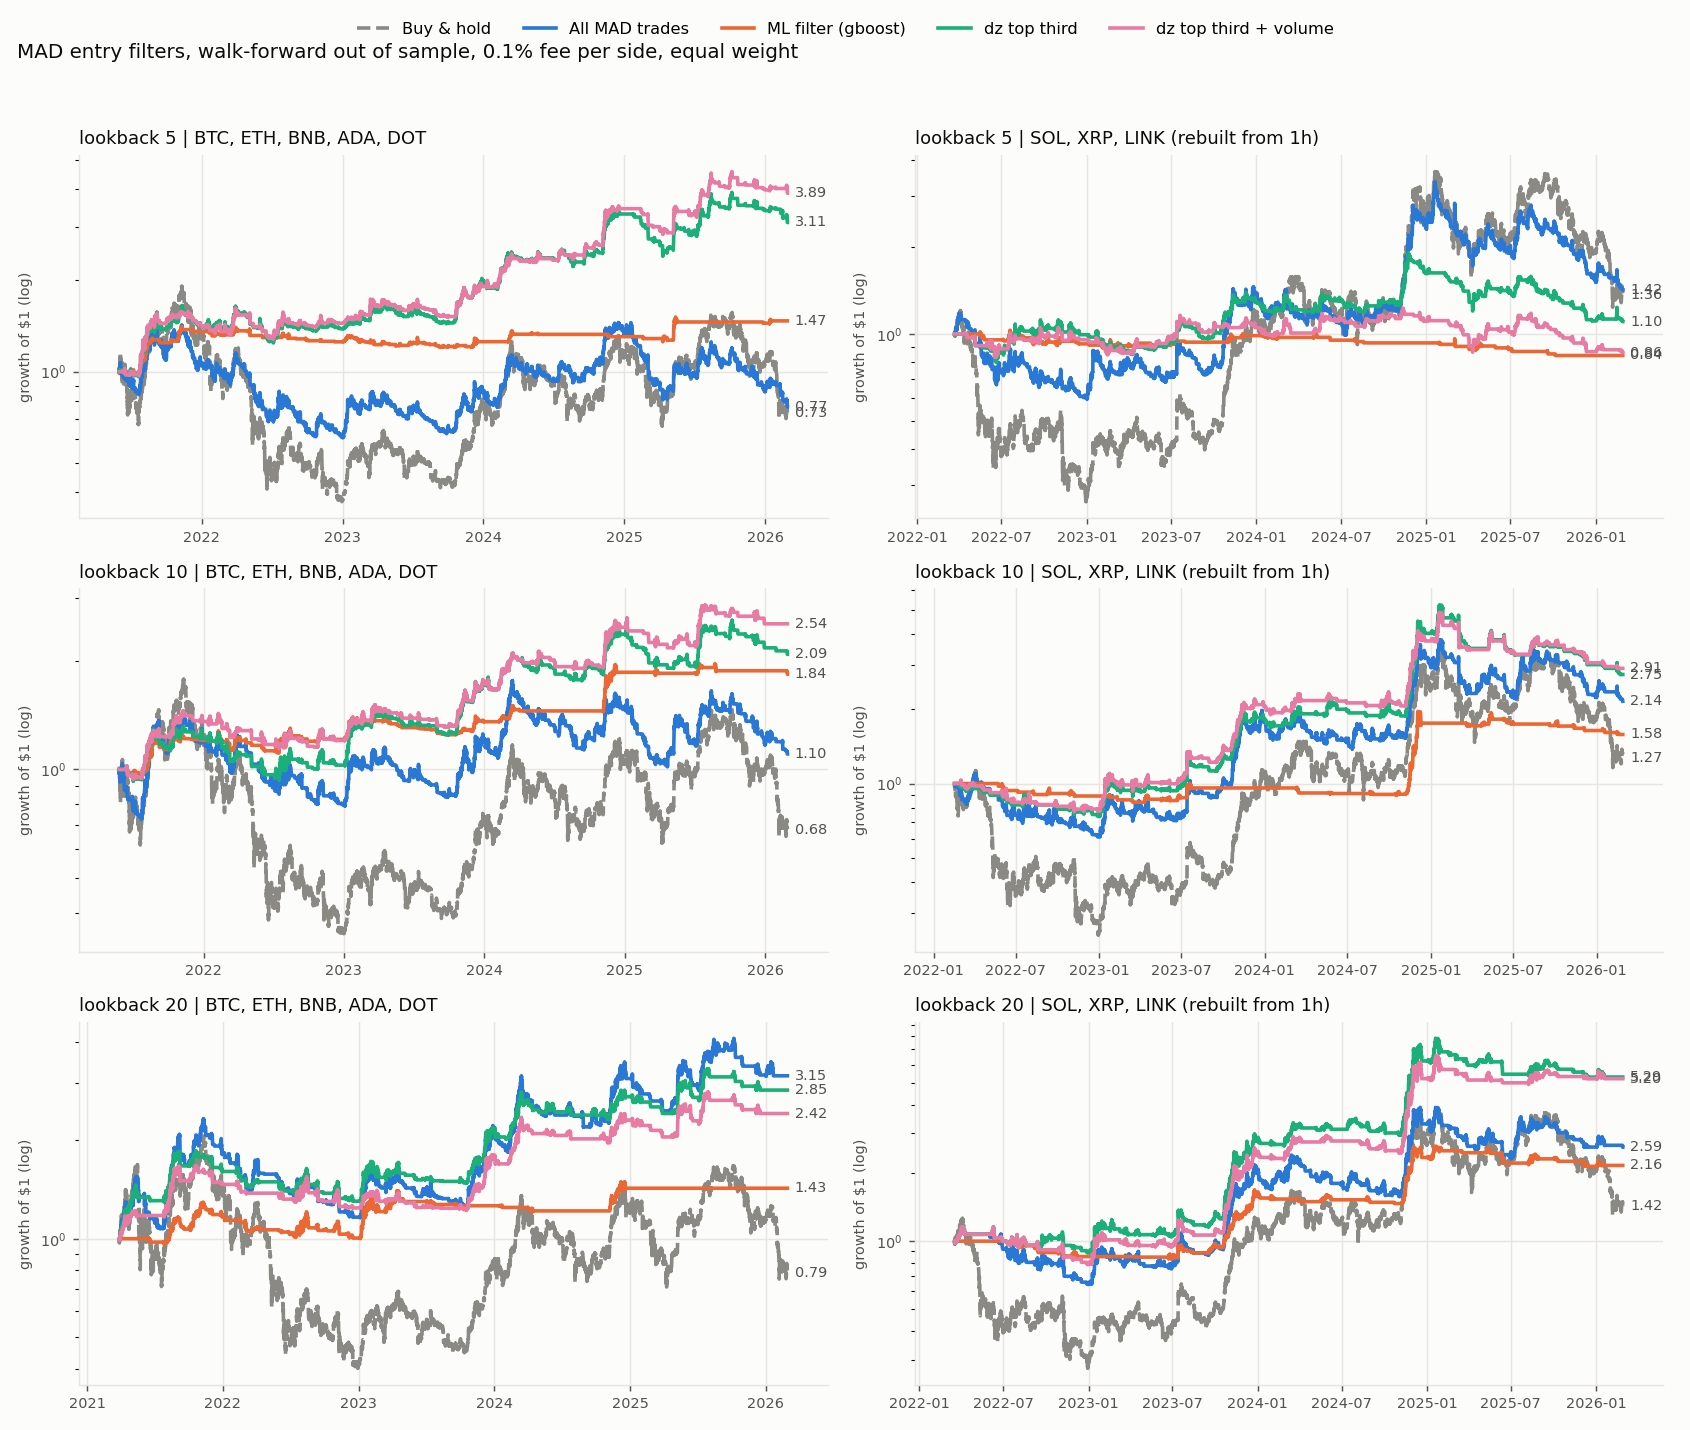
\includegraphics[width=\linewidth]{cumulative_returns.png}
\caption{Growth of \$1 (log scale) for the MAD filters, 4-hour bars, walk-forward. Left column: BTC, ETH, BNB, ADA, DOT (data to 2024 for BNB, ADA and DOT at the time of this run); right column: SOL, XRP, LINK. Dashed: buy-and-hold.
Rows: lookback 5, 10, 20.}\end{figure}

%% =====================================================================
\section{The breakout rule}
\subsection{The 12-variant grid}
Table~\ref{tab:grid} gives the pre-specified grid on the 8 coins, 2018--2026, no fitting. ``Mean net'' is per trade. ``$p$'' is the random-entry test. Sharpe, maximum drawdown and exposure are for the equal-weight portfolio.
``Halves'' are the Sharpe of the first and second half of the sample.

\begin{table}[H]\centering\scriptsize\setlength\tabcolsep{3pt}
\caption{Breakout grid. All 12 variants have $p\approx0$ against random entries. DSR is the weekly-portfolio value with 12 trials.}\label{tab:grid}
\begin{tabular}{rrcrrrrrrcr}\toprule
$k$ & $H$ & Volume & Trades & Mean net & Win & Sharpe & Max DD & Exposure & Sharpe halves & DSR\\\midrule
\rows{tables/breakout_grid.tex}\bottomrule\end{tabular}\end{table}

Every variant earns a positive mean net return, between 0.38\,\% and 2.78\,\% per trade, and beats random entries ($p\le0.003$). The volume filter helps a little at short holds and not at all at $k=12,H=24$
(2.67\,\% without, 2.78\,\% with). Longer holds earn more per trade. The two variants carried forward are the \emph{green} rule ($k=12$, $H=24$, no volume) and the \emph{frozen orange} rule ($k=12$, $H=24$, volume).

\subsection{Robustness checks}
\begin{itemize}
\item \textbf{All 8 coins} have a positive mean net return per trade for both variants (+0.6\,\% to +5.3\,\%).
\item \textbf{Calendar years:} positive in 7--8 of 9 years; weak in 2018 and 2022 (about $-9$\,\% to $+1$\,\% pooled).
\item \textbf{Fees doubled} (0.2\,\% per side): mean net per trade stays at +1.25\,\% and +2.57\,\% for the two best variants.
\item \textbf{Week-block bootstrap, 5th--95th percentile of mean net per trade:} $[+0.9\,\%,+2.0\,\%]$ and $[+1.7\,\%,+3.8\,\%]$.
\item \textbf{MATIC} (renamed, not a survivor): +3.8\,\% and +7.7\,\% per trade, $p=0.02$--0.03.
\item \textbf{Weekly-portfolio DSR} for the $k=12,H=24$ volume rule: 0.997 with 12 trials, 0.956 with 100 and 0.90 with 300. For $k=6,H=12$: 0.99, 0.91, 0.82.
\item \textbf{Forward window} (entries from 28 February 2026, not used to choose the rule): $k=12$ variants are positive (+1.1\,\% to +3.2\,\% per trade, 7 of 8 coins positive); $k=6$ variants are flat to negative.
\end{itemize}
The honest trial count for the whole project is well above 12 (several hundred configurations were tried across MAD, filters and models), so the 100--300 trial values are the fair ones; at those counts the result is borderline rather than clear.

\subsection{Strategy against buy-and-hold: CAGR, Sharpe, drawdown}
\begin{table}[H]\centering\small
\caption{Pooled 8 coins, April 2018 -- October 2026 (8.6 years). Equal weight. Drawdown on 4-hour equity.}\label{tab:cagr}
\begin{tabular}{lrrrr}\toprule
Strategy & CAGR & \$1 became & Sharpe & Max DD\\\midrule
\rows{tables/cagr_full.tex}\bottomrule\end{tabular}\end{table}

\begin{table}[H]\centering\small
\caption{Sub-periods: pooled green and frozen rules against BTC buy-and-hold.}
\begin{tabular}{llrrr}\toprule
Period & Strategy & CAGR & Sharpe & Max DD\\\midrule
\rows{tables/cagr_sub.tex}\bottomrule\end{tabular}\end{table}

\paragraph{Reading.} The green rule roughly matches BTC buy-and-hold on CAGR (35.0\,\% against 33.2\,\%) with about a third of the drawdown ($-26$\,\% against $-77$\,\%) and nearly twice the Sharpe (1.47 against 0.78).
Since 2022 the green rule's CAGR is 21.1\,\% against 12.3\,\% for BTC. The eight-coin buy-and-hold (45.5\,\%) is higher, but it is inflated by survivors such as BNB (63\,\% a year) and SOL (77\,\% a year).
On Bitcoin alone the green rule makes 22.8\,\%, below buy-and-hold: most of its advantage over BTC comes from diversification across eight coins, not from a better Bitcoin signal.
Adding the volume filter (frozen rule) \emph{lowers} CAGR (35.0\,\% to 26.8\,\%) and drawdown ($-26$\,\% to $-21$\,\%).

\begin{table}[H]\centering\small
\caption{Calendar-year returns, pooled 8 coins. 2026 is to 25 October.}
\begin{tabular}{rrrrr}\toprule
Year & Green & Frozen & BTC buy \& hold & 8-coin buy \& hold\\\midrule
\rows{tables/years.tex}\bottomrule\end{tabular}\end{table}

\begin{figure}[H]\centering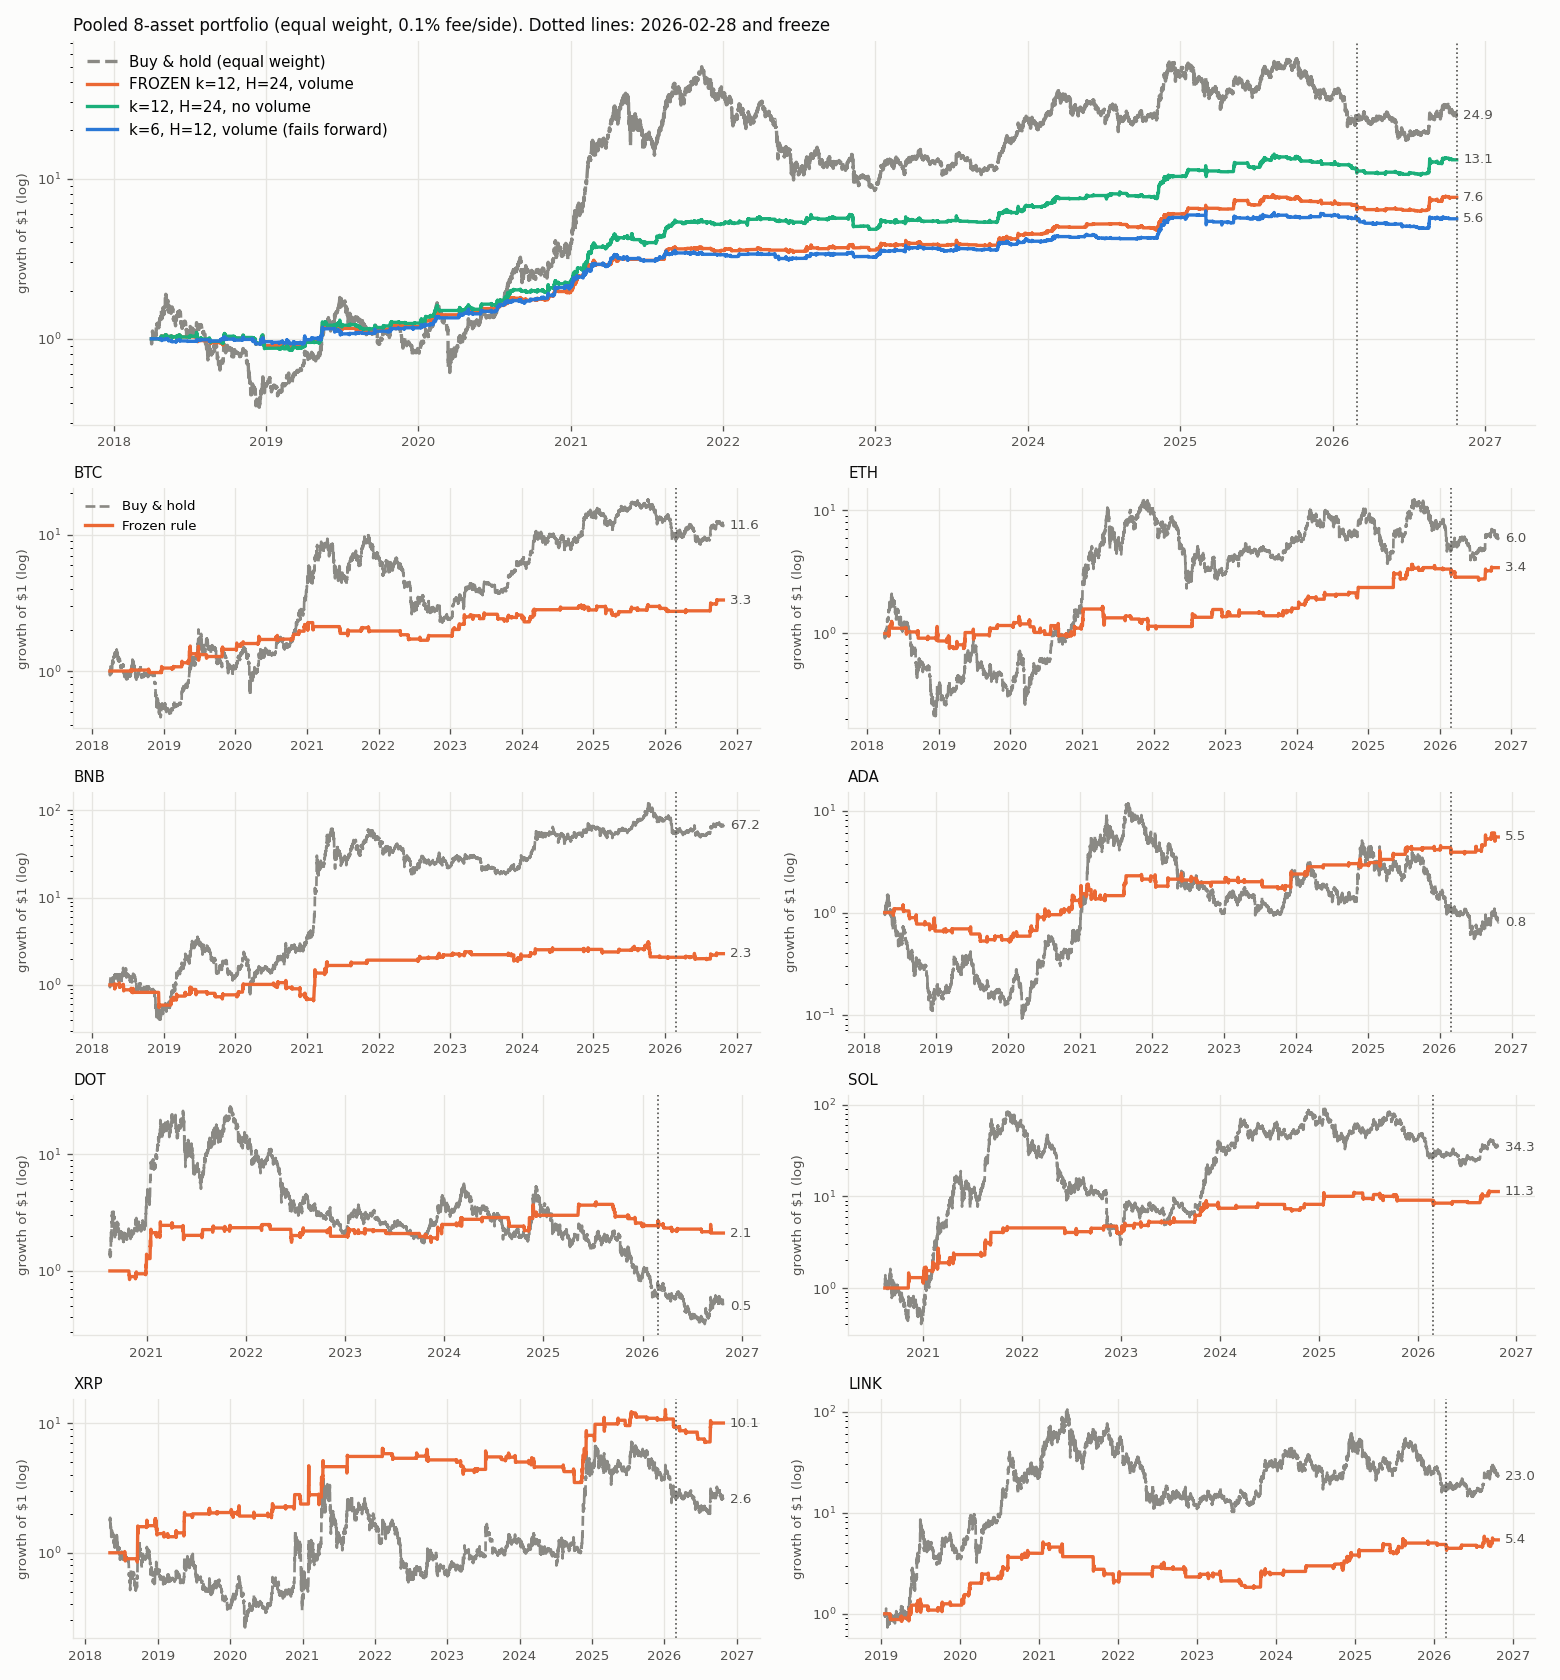
\includegraphics[width=\linewidth]{breakout_curves.png}
\caption{Growth of \$1 on a log scale. Top: pooled 8-coin portfolio for the frozen rule, the green rule (no volume), the faster $k=6$ rule and equal-weight buy-and-hold; dotted lines mark 28 February 2026 and the freeze.
Below: the frozen rule against buy-and-hold per coin. The rule's equity is a series of steps with long flat stretches: it is invested about 10\,\% of the time.}\end{figure}

\subsection{When buy-and-hold loses}
We split each coin's history into calendar years. Table~\ref{tab:lost} gives the frozen rule's average return in coin-years where buy-and-hold lost or gained.
\begin{table}[H]\centering\small
\caption{Frozen rule against buy-and-hold by coin-year. 65 full coin-years across 8 coins.}\label{tab:lost}
\begin{tabular}{lrrrrr}\toprule
 & Coin-years & Mean b\&h & Mean rule & Rule $>0$ & Rule $>$ b\&h\\\midrule
\rows{tables/bh_lost.tex}\bottomrule\end{tabular}\end{table}
\begin{table}[H]\centering\small
\caption{Coin-years in which buy-and-hold lost, by calendar year (averaged over the coins that lost that year).}
\begin{tabular}{rrrr}\toprule
Year & Coins & Mean b\&h & Mean rule\\\midrule
\rows{tables/bh_lost_by_year.tex}\bottomrule\end{tabular}\end{table}
In bear years the rule loses a small amount or gains (2022: $-1$\,\% against $-72$\,\%; 2025: +20\,\% against $-34$\,\%; 2026: +9\,\% against $-22$\,\%). When an asset sits more than 40\,\% below its previous peak (70\,\% of all bars),
the annualised mean return is $-11.7$\,\% for buy-and-hold and +14.8\,\% for the rule. The worst single coin-years still lose (ADA 2018 $-34$\,\%, DOT 2025 $-20$\,\%, SOL 2022 $-12$\,\%), only far less than buy-and-hold.

%% =====================================================================
\section{Per-asset results}
Tables~\ref{tab:bhasset}--\ref{tab:frzasset} give every metric per coin for buy-and-hold, the green rule and the frozen rule over each coin's full history. ``Trades'' and ``Mean net'' are per trade; ``Exposure'' is the share of bars in a position.

\begin{table}[H]\centering\small
\caption{Buy-and-hold per coin, full history of each coin (data to 25 October 2026).}\label{tab:bhasset}
\begin{tabular}{lrrrrrr}\toprule
Coin & Start & Years & CAGR & \$1 became & Sharpe & Max DD\\\midrule
\rows{tables/asset_bh.tex}\bottomrule\end{tabular}\end{table}

\begin{table}[H]\centering\small
\caption{Green rule ($k=12$, $H=24$, no volume) per coin.}\label{tab:greenasset}
\begin{tabular}{lrrrrrrrr}\toprule
Coin & CAGR & \$1 became & Sharpe & Max DD & Exposure & Trades & Mean net & Win\\\midrule
\rows{tables/asset_green.tex}\bottomrule\end{tabular}\end{table}

\begin{table}[H]\centering\small
\caption{Frozen rule ($k=12$, $H=24$, volume spike) per coin.}\label{tab:frzasset}
\begin{tabular}{lrrrrrrrr}\toprule
Coin & CAGR & \$1 became & Sharpe & Max DD & Exposure & Trades & Mean net & Win\\\midrule
\rows{tables/asset_frozen.tex}\bottomrule\end{tabular}\end{table}

\begin{table}[H]\centering\small\setlength\tabcolsep{4pt}
\caption{Side by side: buy-and-hold (B), green (G) and frozen (F) per coin.}\label{tab:side}
\begin{tabular}{l rrr rrr rrr}\toprule
 & \multicolumn{3}{c}{CAGR} & \multicolumn{3}{c}{Sharpe} & \multicolumn{3}{c}{Max drawdown}\\\cmidrule(lr){2-4}\cmidrule(lr){5-7}\cmidrule(lr){8-10}
Coin & B & G & F & B & G & F & B & G & F\\\midrule
\rows{tables/asset_compare.tex}\bottomrule\end{tabular}\end{table}

\paragraph{Reading the per-coin tables.}
\begin{itemize}
\item \textbf{CAGR:} the green rule beats buy-and-hold on ETH, ADA, DOT and XRP, and loses on BTC, BNB, SOL and LINK. It does best where buy-and-hold did badly (ADA $-2.5$\,\% against 44\,\%, DOT $-10.7$\,\% against 13.2\,\%) and worst on the coins that went up most (BNB 63\,\% against 23\,\%).
\item \textbf{Sharpe:} the green rule beats buy-and-hold on 6 of 8 coins (not BNB or LINK). The frozen rule beats it on 6 (not BNB or LINK).
\item \textbf{Drawdown:} on every coin both rules have a smaller drawdown than buy-and-hold ($-26$\,\% to $-66$\,\% against $-77$\,\% to $-99$\,\%). Even so the rules' drawdowns are large on single coins (BNB, LINK, SOL); the pooled $-26$\,\% comes from diversification.
\item \textbf{A single coin is a weak portfolio.} Per-coin Sharpe ratios of the rules are 0.5--1.1; only pooling takes it to 1.4--1.5.
\end{itemize}

\subsection{Year by year, per coin}
Tables~\ref{tab:yrfrz} and~\ref{tab:yrbh} give calendar-year returns for every coin, for the frozen rule and for buy-and-hold. A dash means the coin was not listed for most of that year. 2026 is to 25 October.
\begin{table}[H]\centering\scriptsize\setlength\tabcolsep{3.5pt}
\caption{Frozen rule, calendar-year return per coin.}\label{tab:yrfrz}
\begin{tabular}{lrrrrrrrrr}\toprule
Coin & 2018 & 2019 & 2020 & 2021 & 2022 & 2023 & 2024 & 2025 & 2026\\\midrule
\rows{tables/asset_year_frozen.tex}\bottomrule\end{tabular}\end{table}
\begin{table}[H]\centering\scriptsize\setlength\tabcolsep{3.5pt}
\caption{Buy-and-hold, calendar-year return per coin.}\label{tab:yrbh}
\begin{tabular}{lrrrrrrrrr}\toprule
Coin & 2018 & 2019 & 2020 & 2021 & 2022 & 2023 & 2024 & 2025 & 2026\\\midrule
\rows{tables/asset_year_bh.tex}\bottomrule\end{tabular}\end{table}
The pattern is the same coin by coin: the rule's year-by-year returns are bounded (rarely below $-20$\,\% or above $+60$\,\%, with a few exceptions such as BNB in 2021) while buy-and-hold swings from $-80$\,\% to several hundred per cent.

%% =====================================================================
\section{The frozen rule and its verdict}\label{sec:freeze}
On 25 October 2026 the rule with $k=12$, $H=24$, volume spike above 1.5 times its 50-bar mean was frozen. The script \code{frozen\_breakout.py} stores the parameters, a hash of the code, the freeze time
(first entry that counts: 2026-10-25 20:00) and baselines. It scores only entries after the freeze. Baselines at freeze:
\begin{center}\small\begin{tabular}{lrrrrr}\toprule
Window & Trades & Mean net & Win & Coins $>0$ & Bootstrap 5th pct\\\midrule
Before 2026-02-28 & 529 & +2.75\,\% & 58\,\% & 8/8 & +1.6\,\%\\
28 Feb 2026 $\to$ freeze & 41 & +3.17\,\% & 59\,\% & 7/8 & $-1.6$\,\%\\\bottomrule\end{tabular}\end{center}
The second window was looked at while choosing the rule, so it is \emph{not} out of sample.

\paragraph{Pre-registered verdict.} Wait for at least \textbf{100 forward trades}. \textbf{Accept} if the mean net return per trade is above 0, the week-block bootstrap 5th percentile is above 0, and the random-entry $p$ is below 0.05.
\textbf{Reject} if there are 100 trades and the mean is 0 or below. Otherwise the result is inconclusive. At about 5 trades a month this takes roughly 20 months. First re-score on 25 October 2026: 0 forward trades, inconclusive.

%% =====================================================================
\section{What we got wrong, and caveats}\label{sec:corr}
\begin{itemize}
\item \textbf{The first Deflated Sharpe of 0.98 was inflated.} It counted about 320 pooled trades from correlated coins as independent. On weekly portfolio returns the same rule scored 0.75 (36 trials).
\item \textbf{Earlier claims of ``lower drawdown'' were exposure.} A rule invested 19\,\% of the time has a smaller drawdown than buy-and-hold even without skill. Exposure-matched benchmarks (Table~\ref{tab:exp}) have the same or smaller drawdowns.
\item \textbf{The \code{dz} rule's headline cell did not replicate} on SOL, XRP, LINK for lookback 5.
\item \textbf{Survivorship:} 7 of 8 coins survived. A fair test needs coins that were delisted or went to zero.
\item \textbf{Bull-heavy sample:} 2020 and 2021 contribute most of the return (green: +83\,\% and +128\,\%). Since 2022 the green CAGR is 21\,\%.
\item \textbf{Costs:} 0.1\,\% per side with no slippage, no funding, no spread. Real execution on thin coins will cost more. Idle cash earns nothing in these numbers; a stablecoin or Treasury yield would raise every CAGR.
\item \textbf{Number of trials:} the 12-variant grid was fixed in advance, but it was chosen after a long search through MAD filters and models. The 100--300 trial DSR values are the honest ones.
\item \textbf{Forward evidence:} none yet for the frozen rule.
\item \textbf{Data:} BNB, ADA and DOT 4-hour data from May 2024 to October 2026 and all data after February 2026 come from a different download than the original files; SOL, XRP and LINK history before 2026 is rebuilt from 1-hour bars.
\end{itemize}

\section{Should the strategy be kept?}
\paragraph{Our view.} Keep it as a \textbf{watch-only record}, not a sized position. The evidence is a clear but unconfirmed in-sample signal, a mixed forward window and a pre-registered test that cannot conclude for about 20 months.
If capital were ever used, a small amount that can be lost entirely is appropriate: a few percent, only the large liquid coins, a stop rule written beforehand (for example, switch it off after a 25\,\% fall from its peak or if the first 50 forward trades average below zero), and idle cash in a stablecoin or Treasury bills.
\paragraph{Consistency with the companion \texttt{herc\_llm} research.} That repository's keep list (\code{KEPT.md}) gives a strategy a status only through its own pre-registration, and its closed register records two results that match ours: (a) the ghost Donchian filter on BTC/ETH,
whose drawdown cut ``equals holding less'' (CLOSED \#26), and (b) portfolio algorithms (equal weight, inverse volatility, HRP, HERC, risk parity, minimum variance) over crypto coin sets, closed with 0 of 18 arms passing (CLOSED \#24, ``do not re-propose another algorithm or coin set on today's survivors'').
We therefore \emph{do not} recommend building a HERC/HRP weighting on the coins here; at most it can be tested on a point-in-time universe that includes delisted coins.

\section{What could still be studied}
\begin{itemize}
\item Re-score the frozen rule as bars accumulate (fetch with \code{fetch\_klines.py}, run \code{frozen\_breakout.py}), and decide only at 100 forward trades.
\item Build a point-in-time universe including delisted coins to remove survivorship bias.
\item Volatility-based exit and a market-state gate (for example BTC trend) instead of a fixed 24-bar hold; compare at equal exposure.
\item Risk-targeted sizing per trade across overlapping signals.
\item The same event on other venues, on futures, and with realistic costs on smaller coins.
\item Cluster-aware inference throughout (week blocks across coins), and combinatorial purged cross-validation.
\end{itemize}

\section{How to reproduce}
All code is in \code{src/meta\_labeling/} of the repository, run from the project root with the project virtual environment.
\begin{center}\small\begin{tabular}{p{0.34\linewidth}p{0.58\linewidth}}\toprule
Script & Purpose\\\midrule
\code{fetch\_klines.py} & Append closed 4-hour bars from Binance public klines (backs up originals)\\
\code{resample\_4h.py} & Rebuild 4-hour bars from 1-hour bars\\
\code{run\_meta.py}, \code{run\_meta\_pooled.py} & Meta-labeling with purged walk-forward, permutation control, DSR\\
\code{run\_regime\_study.py} & Equity-curve comparison of regime rules, ML and \code{dz}, random-veto control\\
\code{feature\_importance.py} & Permutation importance of the gradient-boosting model\\
\code{run\_ensemble.py} & Lookback ensemble and exposure-matched benchmarks\\
\code{run\_breakout.py}, \code{run\_breakout\_checks.py} & Breakout grid and robustness\\
\code{frozen\_breakout.py}, \code{frozen\_breakout.json} & Freeze and forward score\\
\code{plot\_breakout.py}, \code{plot\_cumulative.py} & Figures\\
\code{report/build\_tables.py} & Builds the tables in this document\\\bottomrule\end{tabular}\end{center}
The chronological log of every step, with the numbers, is \code{RESEARCH\_LOG.md}.
\end{document}
